%=========================================================================
% (c) Michal Bidlo, Bohuslav K?ena, 2008

\chapter{Introduction}

Ever since the humans inabited the Earth, one of the most important things was to know who they're dealing with using the identity of their partner. Before the spoken word, their identity mainly consisted of how they looked, sounded or maybe even smelled to others.
With the development of languages came names, like ``John Smith'' or ``Maria Garcia'' which, given the tendecy of early populations being small, were sufficient as a form of identity. \\
However, with the dawn of the industrial age people would be moving to cities, creating larger and larger populations and with the creation of factories, employing an increasing number of people, it was important to somehow store and manage
their identities and duties. At first, this was done using paper documents stored somewhere in the factory, but this solution proved to be increasingly difficult as sorting and searching through these documents had to be done manually and this took a lot of time. \\
With the advent of computers, this problem was solved by storing the identities of employees into databases or directory servers, from which they could be retrieved easily if needed.
As the factories turned into companies, spanning multiple buildings, countries, or even continents, and computers becoming smaller, more powerful and generally available, it was important to manage stored identities
and control which parts of the system the company's employees could access given their role using information management software. As a single unwanted change in this identity management could even prove fatal to the whole network, one of the most important parts a identity management system are the notifications of such changes.
These notifications can be then used to respond to the event by the administrator or, more importantly, another automated system.\\
The main topic of this thesis are these notification systems and mechanisms in identity management software, specifically their implementation in the FreeIPA project focusing largely on interopability with third party software.
Chapter \ref{chp:freeipa} will be introducing the reader to the FreeIPA project and its components, while chapter \ref{chp:ad} compares FreeIPA to Microsoft's Active Directory with emphasis on notification mechanisms.
Chapter \ref{chp:anal} will be looking at the proposed use cases for the notification system and, last but not least, chapter \ref{chp:appDesign} will tackle the issues of notification sending function placement and method of transfer, as well as providing an early design of the system.

\chapter{FreeIPA}
\label{chp:freeipa}

FreeIPA (where IPA stands for Identity, Policy and Audit) is an open-source security management solution sponsored by Red Hat aimed primarily at Linux and Unix machines \cite{ipaWeb}.

The project itself combines a number of various existing open-source technologies to achieve the goal of providing centralized authentication and authorization, as well as storing important account information like users or group memberships.
FreeIPA also aims to provide easy management and setup of a domain controller which would otherwise be very difficult by using the same components on your own.

This chapter will briefly introduce some of the components FreeIPA uses and describe the architecture of the resulting FreeIPA server solution, including the posibilities of extending the project.

\section{Directory Server}
FreeIPA's directory service is the foundation of the project as it stores various information on behalf of all of FreeIPA's components.
It also plays a big role in authentication and authorization using Kerberos which will be presented in the next section.

The LDAP protocol \cite{ldapRFC} is used as a mean of communication with the server and the data itself is stored in a Directory Information Tree (DIT) which is a tree-like data structure.
An example of a DIT structure can be seen in figure \ref{fig:dit}.

\begin{figure}[!ht]
    \centering
        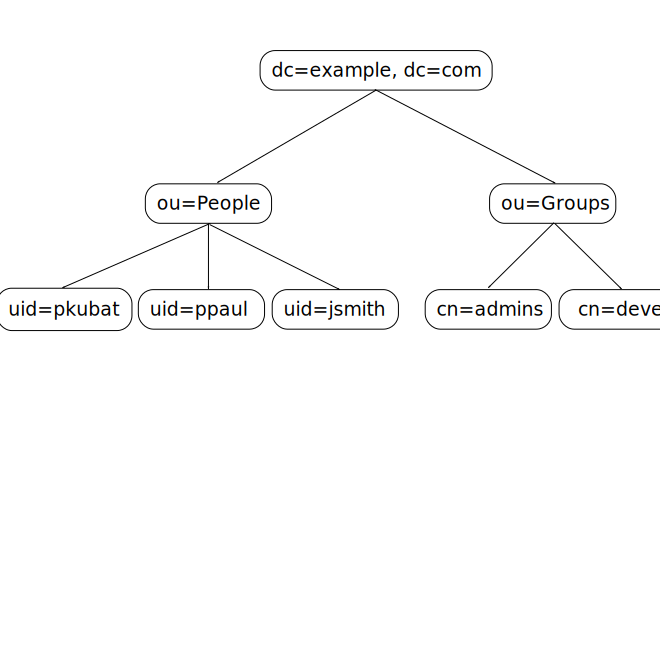
\includegraphics[scale=0.6]{fig/ldap-dit}
    \caption{LDAP Directory Information Tree}
    \label{fig:dit}
\end{figure}

\clearpage
LDAP provides several operations to use with the server \cite{ldapRFC}:

\begin{itemize}
    \item \textbf{add, delete, modify:} These operations add, remove and modify the data contained in the DIT.
    \item \textbf{search, compare:} The search and compare operations are used in querying the DIT for specific information.
    \item \textbf{bind, unbind, abandon:} These operations can be used to authenticate to the directory, terminating the connection or abandoning a previously sent request entirely, respectively.
    \item \textbf{extended operations:} New operations that are not a part of the original protocol.
\end{itemize}

The actual LDAP compatible server contained in FreeIPA is implemented using the 389 Directory Server project \cite{ldapWeb}.
% TODO: ACLs

\section{Kerberos}
Kerberos \cite{kerbRFC} is a network authentication protocol that uses symmetric encryption using a pre-shared key to authenticate a client to a network service (and vice versa) via an insecure connection using a trusted third party service called a Key Distribution Center (KDC). \\
The resulting communication is secure because no secret keys are transported over the network in plaintext format as the KDC already contains a database of credentials for users and services in the Kerberos realm. \\

\begin{figure}[!ht]
    \centering
        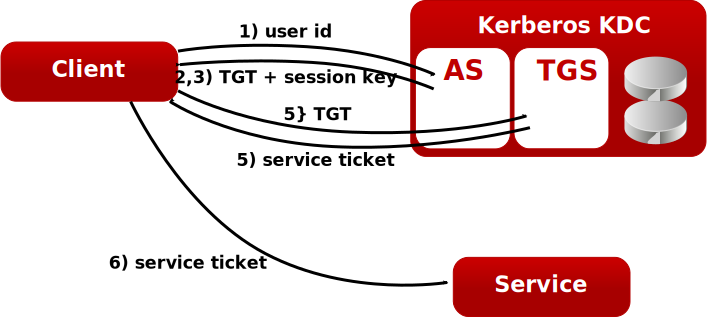
\includegraphics[scale=0.6]{fig/kerb}
    \caption{Kerberos authentication process}
    \label{fig:kerb}
\end{figure}

The process of authenticating the user to a network service is shown in figure \ref{fig:kerb} and can be described in these steps:
\begin{enumerate}
    \item The user sends his principal name (an unique identifier) to the KDC's Authentication Server (AS) via a plaintext request.
    \item The AS then checks the database to make sure the user exists and sends back a randomly generated session key to be used to encrypt communication with another service called a Ticket-Granting Service (TGS) encrypted with the user's secret key.
    \item The AS also generates a set of credentials called a Ticket-Granting Ticket (TGT) which includes the previously generated session key and is encrypted by the secret key of the TGS.
    \item After recieving the first message the client decrypts it using his secret key. This is the only time the user's key is actually used. The TGT which the client can't decrypt himself is saved in a cache on the client's side to be used later to setup a session with the TGS. At this point the user is authenticated to the Kerberos realm and doesn't have to input his secret key again for a set amount of time (commonly 10-24 hours).
    \item When the user wants to authenticate agains a service in the Kerberos realm he just has to ask the TGS to send him a ticket. This request is encrypted using the session key created in previous two steps.
    \item The user then authenticates to the chosen service using this ticket without the need for his secret key.
\end{enumerate}

As the security of the Kerberos protocol is partly based on the time stamps of tickets, all of the clients and services in the realm have to be properly synchronized time-wise.
To achieve this goal the Network Time Protocol can be used in the FreeIPA project. \\
FreeIPA's KDC is implemented using the MIT Kerberos \cite{kerbWeb} open source software and FreeIPA also provides its own KDC data backend called ipa-kdb which is used to both read and write user information to FreeIPA's LDAP directory service \cite{kerbIpa}.
\section{DNS}
Even though it would be possible to access network services located in a FreeIPA domain directly using their IP addresses, it is much more easier to do so using domain names. \\
The Domain Name System (DNS) \cite{dnsRFC} is distributed naming system, that translates domain names, which can be easily memorized by humans, into IP addresses using special name servers.
As such if one wants to access a network service or a webpage he doesn't have to remember its IP address, only the IP address of the name server (which is stored localy on the client machine) and the domain name of the service/webpage. \\
The domain name space resembles a tree structure, each node having a label that designates a part of its domain name, while the full domain name of the node can be built by concatenating this label with the domain name of its parent node. \\
The name space is divided into zones starting at the root of the tree structure with child nodes of the root node called top-level domains (TLD).

\begin{figure}[!ht]
    \centering
        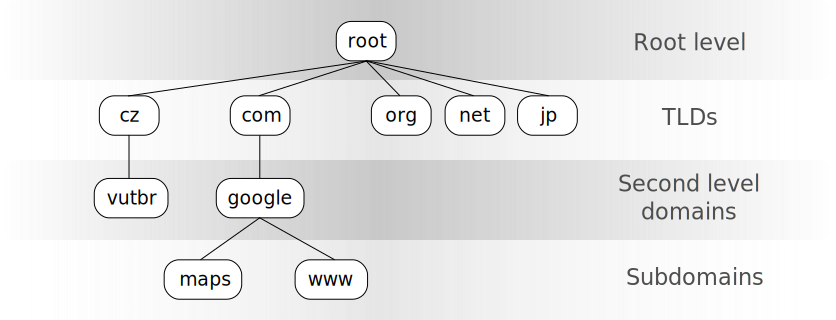
\includegraphics[scale=0.6]{fig/dns-tree}
    \caption{Domain name space}
    \label{fig:dnsTree}
\end{figure}

These zones can contain one or several domains, each domain served by one or several name servers, and can be divided into additional zones if deemed necessary. \\
The DNS server in FreeIPA uses an enhanced BIND name server which allows FreeIPA to store data into an LDAP directory \cite{dnsIpa}.
However using FreeIPA's integrated DNS server is optional and as such the project can be used with a different third party DNS server if so desired.

\FloatBarrier
\section{FreeIPA Architecture}
While the most important components of the FreeIPA project have been described in previous sections, a number of components are still missing for the infrastructure to be complete.

\begin{figure}[!ht]
    \centering
        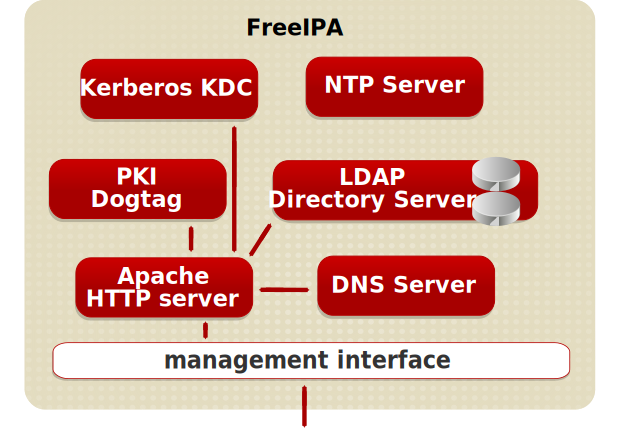
\includegraphics[scale=0.6]{fig/ipa-architecture}
    \caption{High level FreeIPA server architecture}
    \label{fig:ipaHigh}
\end{figure}

To start with, FreeIPA can optionally use the \textbf{Dogtag project} \cite{certWeb} as an integrated Public Key Infrastructure that signs and publishes certificates for hosts and services inside the domain. \\
Secondly, the \textbf{Apache Web Server} is used to provide web based access to the management APIs using the XML-RPC and JSON-RPC APIs as well as to serve the web interface to the clients. \\
And last but not least, as one of the most important additions to the project, FreeIPA's \textbf{ipalib} framework is used together with the Command Line and Web based interfaces to administer the FreeIPA domain. \\
A high level and a detailed representation of the resulting infrastructure can be found in figures \ref{fig:ipaHigh} and \ref{fig:ipaDetail}, respectively.

\begin{figure}[!ht]
    \centering
        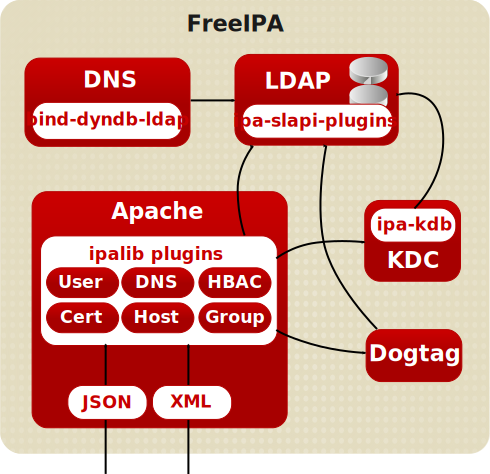
\includegraphics[scale=0.6]{fig/freeipa-detail}
    \caption{Detailed look at FreeIPA architecture}
    \label{fig:ipaDetail}
\end{figure}

The ipalib framework is written using the Python programming language and is highly modular -- most if not all of its functionality is implemented using plug-ins, which are executed on demand using the Apache Server.
This framework is generally used to connect the isolated components into the FreeIPA solution, providing the ability to enroll users or services into the domain, managing the certificates used within the domain or
adding Host Based Access Control rules for even beter access management.

\section{Extending FreeIPA}
\label{sec:ipaExt}

\subsection{Extending the Framework}
As previously stated, the ipalib framework is highly modular and extensible with a couple of different ways to add new (or modify current) functionality \cite{extIpa}:\\
First off one can directly extend existing objects of the ipalib framework. These objects are mainly responsible for executing various commands sent using the XML and JSON APIs
and as such extending or modifying the objects, eg. adding a parameter or rewriting an object's label, can alter the default behaviour of those commands. \\
The second way is to extend methods of an object stored in the LDAP database by adding callbacks to these methods.
Callbacks are user-defined functions that are called at various stages of exectution of the method:
\begin{description}
    \item[Pre callback]\hfill \\This callback is called before executing the method's code. Used for modifying arguments and data validation.
    \item[Post callback]\hfill \\This callback is called after executing the method's code and allows for analyzing the result of the command.
    \item[Exc callback]\hfill \\This callback is called in case there is an error during the execution of the method's code. Can be used to recover from the error.
    \item[Interactive callback]\hfill \\Allows a command to decide if additional parameters should be requested from the user.
\end{description}
\subsection{Extending the Directory Server}
The 389 DS used in the FreeIPA project has two ways of creating extensions for its operations, first one achieved by writing a server plug-in, while the second one uses LDAP's Content Synchronization Operation protocol.
\subsubsection{Server Plug-ins}
There are several types of plug-ins that can be used when trying to extend the directory server \cite{extLDAP}:
\begin{description}
    \item[Pre operation]\hfill \\A pre operation plug-in is executed before starting the LDAP operation. Mostly used for data validation.
    \item[Post operation]\hfill \\A post operation plug-in is executed after performing the LDAP operation. Can be used for notifications.
    \item[Entry storage and fetch]\hfill \\Executed before writing and reading data from the database, respectively. An example of this type of plug-in would be encryption/decryption of data saved in the database.
    \item[Extended operation]\hfill \\Executed when the client calls an extended operation.
    \item[Syntax]\hfill \\Run when getting a list of candidates for a search. Can be used to modify comparison operations.
    \item[Matching rule]\hfill \\Run when the client sends a request with an extensible matching search filter.
\end{description}
One can see that there are some similarities to callbacks of ipalib's extensions, especially the way of calling pre and post operations plug-ins is basically the same as pre and post callbacks
differing only in when they are called. While pre and post callbacks are bound to a specific method of a specific command object (eg. before or after executing a user-add command),
the pre and post operations plug-ins are bound to an LDAP operation and as such are run much more frequently.

\subsubsection{Content Synchronization Operation}
\label{subsec:syncrepl}
The Content Synchronization Operation (syncrepl) is an extension of the existing search operation provided by LDAP and is mostly used, as its name implies, as a mean of directory content synchronization across different applications.
The operation can be configured to provide a client with changes made to a subtree of a DIT and can be used similarly to 389DS's pre/post operations without the need to extend the whole add/modify/delete operation.
As syncrepl extends the search operation the client can use its content control attributes to specify the content changes it wants to recieve, namely base DN and search scope to control the scope of the operation and filter
to further specify which entries' changes the client is interested in.\\
After using the syncrepl operation (with refreshAndPersist mode) the client is sent initial content located in the DIT after which the server will only send notifications about changes within the tracked content. Updates in the DIT can generate add, modify and delete result messages according to the changes made and
upon recieving these changes the client has to determine the differences by himself as the server will send all of the entry's attributes on its modification (in case of add or modify state change) or none at all (in case of delete state change).\\
Syncrepl also offers a polling (refreshOnly) mode, which allows the client to poll for changes at his own discretion. This mode however will not be used in this thesis and is thus only mentioned for the sake of completeness.
\chapter{Active Directory}
\label{chp:ad}

\section{Structure and Components}
This section is based on the official documentation for Active Directory (AD) \cite{ADoverview}.\\
AD is a distributed directory service used by the Microsoft Windows Server operating systems and, while similar in the components used, is quite different to the FreeIPA project.\\
Objects located in a AD organized network are structured into a logical structure, the basis of which form forests and domains. \\
\textbf{Forests} are the security boundaries of the logical structure and can be structured to provide data and service autonomy and isolation, removing the dependency on physical topology. \\
Each forest is able to hold several \textbf{domains}. These domains can be structured to provide data and service autonomy but not isolation as to allow for replication optimalization.
This logical structure can also be used to control access to data for each domain seperately.

\begin{figure}[!ht]
    \centering
        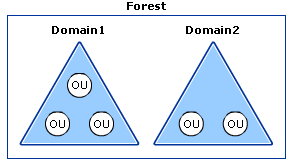
\includegraphics[scale=0.6]{fig/AD-forest}
    \caption{An Active Directory forest and its domains \cite{ADoverview}}
    \label{fig:adForest}
\end{figure}

Each domain is connected to one or more \textbf{domain controllers}. A domain controller is a service that stores directory data and manages user and domain interactions.
Each domain controller consists of a \textbf{schema}, which defines objects and attributes that can be store in the directory, a \textbf{data store}, which manages the storing and retrieving of data, and the actual \textbf{database}.
The data store uses a number of interfaces to access stored data as can be seen in figure \ref{fig:adController}, one of which is the same protocol as the 389DS uses in FreeIPA -- LDAP.

\begin{figure}[!ht]
    \centering
        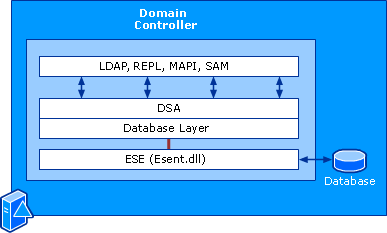
\includegraphics[scale=0.6]{fig/AD-controller}
    \caption{Active Directory Domain Controller \cite{ADoverview}}
    \label{fig:adController}
\end{figure}

Active Directory also uses, similarly to FreeIPA, DNS as its domain controller location mechanism and Kerberos for user authentication.

\FloatBarrier
\section{Notification Mechanisms}
\label{sec:adNotif}
As AD does not by itself provide a complete notification system, this section describes mechanisms contained in AD and Windows operating systems in general that can be used to send notifications between applications. \\
The following mechanisms are available for users of AD directory service:

\begin{description}
    \item[Change Notifications]\hfill \\
        This mechanism allows for a client to register with a domain controller to recieve notifications for changes in the AD domain service. The notification control is specified in a LDAP asynchronous search
        operation. \\
        The user can define a number of search parameters: scope, to monitor just the object or its immediate children, filter, which allows for object filtering and
        attributes, a list of the changed object's attributes that will be returned \cite{ADtrack}.\\
        This mechanism is very similar to the syncrepl operation described in \ref{subsec:syncrepl}, the only difference being that AD allows the client to configure which attributes of the object he wants returned
        while syncrepl only returns all of the attributes.
    \item[Polling]\hfill \\
        The second notification mechanism available in AD is directly polling the AD directory service for changes.
        There are two types of polling available. Polling using Directory Synchronisation control, which is an LDAP server extension that allows to check for changes since a previous state,
        while the other type -- querying using a special uSNChanged attribute -- is used when Directory Synchronisation is unavailable or inefficient \cite{ADtrack}.
\end{description}

These mechanisms are, however, primarily used to mantain consistency of data between the AD directory service and other applications \cite{ADtrack}.
As such there is one additional mechanism that can be used not only with AD, but generally with any application running on a Windows operating system and that is \textbf{Event Tracing}(ET) \cite{ADtrace}. \\
ET is a mechanism that allows for application defined events to be logged into a log file and optionally recieved by other applications in real time.
ET has three major components:%, as can be seen in figure \ref{fig:adTracing}:
\textbf{controllers}, that control the ET sessions, \textbf{providers} that write events into a ET session and \textbf{consumers} which consume one or more event sessions either directly or from a log file.

%\begin{figure}[!ht]
%    \centering
%        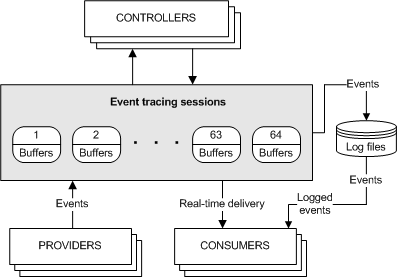
\includegraphics[scale=0.6]{fig/ad-tracing}
%    \caption{Event Tracing model\cite{ADtrace}}
%    \label{fig:adTracing}
%\end{figure}

\chapter{Use Case Analysis}
\label{chp:anal}
In this chapter the author analyses potential use cases of the notification system based on the research of both Active Directory and FreeIPA projects.

\section{Active Directory Use Cases}
As mentioned in section \ref{sec:adNotif} notification systems integrated in Active Directory (change notifications and polling) have generally only one use and that is \textbf{keeping data integrity} between applications that use a copy of data
stored in the directory server and the actual directory server. Even though this use case is not the primary use of FreeIPA's notification system, similar behaviour could be easily introduced
by sending changed data with every generated notification. \\
When it comes to the general event tracing mechanism of the Microsoft Windows Server, it is mainly used for \textbf{logging purposes} by a myriad of applications running on the server.
One of the most interesting of these logs is the \textbf{security event log}. This session logs various security related issues such as every successful/failed login attempts, group membership changes
or failed access attempts to secured objects. \\
Additionaly, while researching Active Directory's notification mechanisms a specific use case for user written scripts came up repeatedly and that is \textbf{password expiry notifications}.
As AD notifies the user of this fact only as he tries to log in with his expired password, said scripts monitored the password expiry time by using a polling mechanism for the expiry attribute and notified the user directly via email.
As such notification on password expiration should be one of the primary use cases of FreeIPA's notification system.
However, as being notified on every login/logout or group membership change would be unnecessary and maybe even bothersome, the system should instead notify on an action with possibly malicious intent,
eg. \textbf{repeated login attempts} or the \textbf{addition of a user into a highly priviledged group} (admins, sales, etc.).
\section{FreeIPA Use Cases}
This section describes the use cases as suggested by FreeIPA's community. \\
Some of the use cases proposed by the community in the project's specification intersect with use cases resulting from the analysis of Active Directory's use cases (user password expiration, group membership changes and repeating login attempts) in the previous section.
Use cases not yet mentioned are as follows:
\begin{description}
    \item[User enrollment, deletion, edit]\hfill \\
        User enrollment (and generally user-based operations) are one of the most frequent and thus important events in a identitz management software.
        As such a notifications of such changes sent possibly via email could be beneficial to some groups (HR, sales). \\
        Additionaly, using this notification system, an automated system could help setup, or delete, user related environments in the system (eg. home folders) on user creation or deletion, respectively.
    \item[Certificate creation/expiry]\hfill \\
        As the Certmonger client-side daemon already takes care of monitoring certificate expiry and optionally their renewal, this use case would be mainly about sending a notice to the concerned groups
        about the impending situation. However, in environments not running Certmonger on the client machines, it could be used to connect to another automated renewal system.
\end{description}

\chapter{Notification System Design}
\label{chp:appDesign}
In this section the author introduces some of the possible approaches for designing a notification sending system in FreeIPA, discussing their positives and negatives while deciding on the details
of the eventual design of the system.
\section{Sender Placement}
\label{sec:sendPlace}
Given the current extensibility of the project as described in section \ref{sec:ipaExt},
there are four possible general placements that can be used:

\begin{enumerate}
    \item Notifications sent directly from the 389DS would allow for the notifications to be delivered even when using an LDAP client different from the FreeIPA client which is apparently quite common.
    However, adding code directly to the directory server (using the plug-in system) might cause drops in performance.
    \item Notification senders located in the ipalib framework would allow for more precise calls of notification sending methods and possibly better performance.
    This approach would also provide the user with the ability to send notifications that would not be limited to changes in the 389DS.
    \item A hybrid approach that combines the previous two approaches and thus adds senders to both the 389DS and the ipalib framework for different operations depending on the severity of hits on performance.
    \item A notification sending extension located in the ipalib framework together with a simple syncrepl using monitoring daemon would have the same advantages as the hybrid plug-in approach without influencing
    the 389DS directly.
\end{enumerate}
\clearpage

While there are no ready-made recievers contained in Active Directory that could help with the choice of approach, it still offers valuable information on what properties the receivers (and senders) should have:

\begin{description}
    \item[Generalization]\hfill \\
        All of AD's available notification mechanisms use a general user-defined notification reciever.
        This allows the user to have control over how the notifications will be processed and responded to.
    \item[Variety]\hfill \\
        AD offers the user a number of different ways of sending notifications. As such the user can decide if he wants to recieve notifications any time an attribute is changed,
        or if he wants to check for changes himself periodically.
\end{description}



\section{Method of Communication}

There are many different protocols that can be used for the actual notification transfer, like the Advanced Message Queuing Protocol or Fedora's own Fedora Infrastructure Message Bus,
however the \textbf{D-Bus message system} has been chosen by the author as the method of transfer.\\
The D-Bus message system is a communication mechanism between processes running on the same host that is present on nearly any Linux operating system,
which is one of the reason thats make it so attractive to be used as the transport medium for notifications in FreeIPA.
The architecture of the D-Bus system is quite similar to Microsoft's Event Tracing mechanism, with the difference of D-Bus not logging sent messages in a file.
The architecture consists of a \textbf{dbus daemon} running the actual bus and individual \textbf{processes}, who can each send and recieve messages over the bus.
D-Bus messages are transported over the bus by the dbus daemon, to which any number of processes can be connected at any given time \cite{dbusWeb}. \\
D-Bus offers two different way to send messages between processes:
\begin{description}
    \item[Method calls]\hfill \\
        The communication using method calls over D-Bus occurs between exactly two processes, one of which takes on the role of the server (exporting methods), while the other is a client (calling methods).
        This way of message transfer allows for a reply to be sent back to the server by the client. This reply could be used as a way to determine whether the notification-related action on the recieving end
        was carried out without any issues and log the resulting error codes and messages if there are any.\\
    \item[Signals]\hfill \\
        Using signals as the way of communication it is possible to send messages from a single server process to any number of listening client processes. However, as the communication is only one-way
        this means there is no way of replying back to the server after the client's signal handler finishes.
\end{description}
While using signals allows the process to broadcast messages, the decision which approach to use basically boils down whetether the sending side is interested in reacting to what happens on the recieving side or not,
as the broadcasting ability can be emulated using a middle-man process to transform the method call into a signal if necessary. After discussing the question which approach to adopt with the FreeIPA community, the author has decided to use
method calls with return values being used for logging purposes on behalf of FreeIPA. \\
D-Bus also has APIs (bindings) written in a number of languages, including the \textbf{C and Python languages} used by 389DS and ipalib framework, respectively, for both the sending and recieving side.
Together with the bus being able to send messages from multiple sources, to multiple recievers, this allows D-Bus to be used with any of previously mentioned sender placements, including the hybrid one. \\
There were some concerns that by using D-Bus, any change to the data sent to the recievers would mean the need to rewrite the reciever to accomodate to the changes made.
However, using the Python bindings and its argument type discovery function, it should be possible for the reciever to work even after the changes have been introduced to the senders.
In case the reciever is written in another lower-level binding, the reciever will have to be editted accordingly, but that is to be expected. \\
%Figure \ref{fig:arch} shows the resulting notification system architecture using D-Bus as the method of transfer.

\section{Performance Analysis}
The directory server, being the heart of the whole FreeIPA project, is highly susceptible to performance hits which some of the approaches discussed \ref{sec:sendPlace} might introduce.
With this in mind the author has implemented a basic suite of time measurement tests to map the difference between each of the approaches using minimalistic sender plug-ins located in the ipalib framework and the 389DS directory server.
Both of these test plugins have been implemented using the respective APIs as described in \ref{sec:ipaExt}, and were designed as post operation plugins sending simple notifications to a reciever (also written in Python) using D-Bus method calls as the medium. \\
The tests themselves have been implemented using Python as this allowed for them to be used directly with FreeIPA's ipalib framework, bypassing the overhead of its CLI interface. A total of three tests suites have been prepared --
two for each of the basic approaches, ipalib and 389DS respectively, and a third one for time measurement of an unmodified version of FreeIPA. The result of these tests can be seen in table ??. \\

\section{Monitoring Daemon Design}
To accomodate for some of the use cases proposed in chapter \ref{chp:anal}, a \textbf{lightweight monitoring daemon} will be designed and implemented to be used to check the expiry date of users' passwords and certificates
and send notifications to the bus when necessary. \\

\chapter{Notification Reciever Design}

\chapter{Conclusion}
The aim of this thesis was to introduce the reader to the FreeIPA identity management solution, its components and management framework, and its need for a notification system that would allow for a better administration.
The FreeIPA project was then compared to another identity management system, for which Microsoft's Active Directory was selected, with focus on the analysis of its notification mechanisms and cases in which they are used.
This has however proven to be quite a difficult task as the uses of Active Directory's notifications were found to be quite limited.\\
Additionaly an early look on the coming design of FreeIPA's notification was presented, mainly focusing on placement of notification sending parts of the system and the way of transport of those notifications.
As part of describing the design decisions behind the transport of notifications, the D-Bus message system was introduced to the reader.\\
With this task complete, the author will now discuss the results presented in this thesis with the FreeIPA community, choose which use cases to use in the final system based on their feedback and after that focus on completing its design.\\
Another very important task is the testing of effects of various sender placements on the performance of FreeIPA and its components, as described in chapter \ref{chp:appDesign}.
This testing will be worked upon in tandem with the design of the notification sending part of the system and is expected to have a strong influence on the way the system will be designed.

%=========================================================================
